% "THE BEER-WARE LICENSE" (Revision 42):
%
% <timklge@wh2.tu-dresden.de> wrote this file. As long as you
% retain this notice you can do whatever you want with this stuff.
% If we meet some day, and you think this stuff is worth it,
% you can buy me a beer in return - Tim Kluge

\documentclass[12pt,landscape]{article}
\usepackage{multicol}
\usepackage{calc}
\usepackage{delarray}
\usepackage{amssymb}
\usepackage[landscape]{geometry}
\usepackage[utf8]{inputenc}
\usepackage{color}
\usepackage[compact]{titlesec}
\usepackage{graphicx}
\usepackage{listings}

\pagestyle{empty}
\geometry{top=1cm,left=1cm,right=1cm,bottom=1cm}

\makeatletter

\makeatother
\setcounter{secnumdepth}{0}

\begin{document}

\footnotesize
\begin{multicols}{3}

\begin{center}
     \Large{\textbf{Einführung in die Medieninformatik}} \\
     \small{Für EMI im 1. Semester beim Bart}
\end{center}

\section{Allgemeines}
\subsection{Aufgabenstellungen}
Berechenbarkeit (Lösen mathematischer Probleme), Unberechenbarkeit, Curchsche These (Gleichwertigkeit aller Maschinenkonzepte), Chomsky-Hierarchie (Zusammenhang Automaten <-> Sprachgrammatik), Programmkomplexität, Programmverifikation
\subsection{Medienkompetenz}
Medialitätsbewusstsein + Medienwissen, Medienspezifisches Rezeptionsmuster, Medienbezogene Genussfähigkeit (Bedürfnis nach Identifikation und Unterhaltung), Medienbezogene Kritikfähigkeit.\\
Medien: Mittel zur Speicherung von Information (Physisch oder Format, Text, Video, Audio, )
\section{Text und HTML}
\subsection{Zeichensätze}
Zeichensatz definiert Zuordnung von Zahlen zu Zeichen.
\begin{enumerate}
\item \textbf{ASCII}: 7-bit-Zeichensatz (128 Zuordnungen), 0-31 Steuerzeichen. Neuere Zeichensätze sind meist abwärtskompatibel (Erste 128 Zuordnungen entsprechen ASCII)
\item \textbf{ISO-8859-1, ISO-8859-2 ... ISO-8859-16}: 8-bit-Zeichensätze (256 Zuordnungen), 0-127 ist ASCII, darüber Sonderzeichen wie deutsche Umlauts (-1: Latin1 westeuropäisch, -2: Latin2 osteuropäisch, -5: Kyrillisch, -6: Arabisch, -7: Griechischi [...], -15: Westeuropäisch mit Eurozeichen)
\item \textbf{Unicode}: Internationaler Zeichensatz. Verschiedene Standards: UCS-2 mit 2 hoch 16 Zeichen, UCS-4 mit doppelt so vielen Ebenen. Unicode 5 kennt 99k Zeichen.\\
Unicode-Formate:
\begin{itemize}
\item \textit{UTF-32}: Immer 4 Bytes für ein Zeichen
\item \textit{UTF-16}: 2 Bytes pro Zeichen mit Möglichkeit für mehr, wenn in ersten 2 Bytes spezille Surrogate-Kodierung benutzt wird
\item \textit{UTF-8}: Wichtigstes Unicode-Format, weit verbreitet z. B. für XML. Besteht aus einem Byte pro Zeichen, das nur ASCII ist, wenn das oberste Bit gesetzt ist, ansonsten gehören die nächsten Bytes auch mit zum Zeichen, dann 2-4 Bytes. Aufbauschema: \\
Höchstes Bit ist nicht gesetzt, wenn es nur ein ASCII-Zeichen ist und somit nur aus einem Byte besteht. Ist das höchste Bit gesetzt, gibt die Anzahl der dann folgenden Bits die 1 sind an, aus wie vielen Bytes das Zeichen besteht. Ist das erste Byte z. B. 11100000, folgen noch zwei weitere Bytes für das gleiche Zeichen. 
\end{itemize}
\end{enumerate}
\subsection{Braille-Schrift}
Von Louis Braille 1820 für Blinde entwickelt, für viele natürliche Sprachen verfügbar. Gibt Zeichen als fühlbare Punkte auf dem Papier wieder (6 - 8 Punkte kodieren ein Zeichen). Spezielle Schreibweisen für Formeln, Musik o. ä.
\subsection{Schrift}
\subsection{Eigenschaften}
\begin{center}
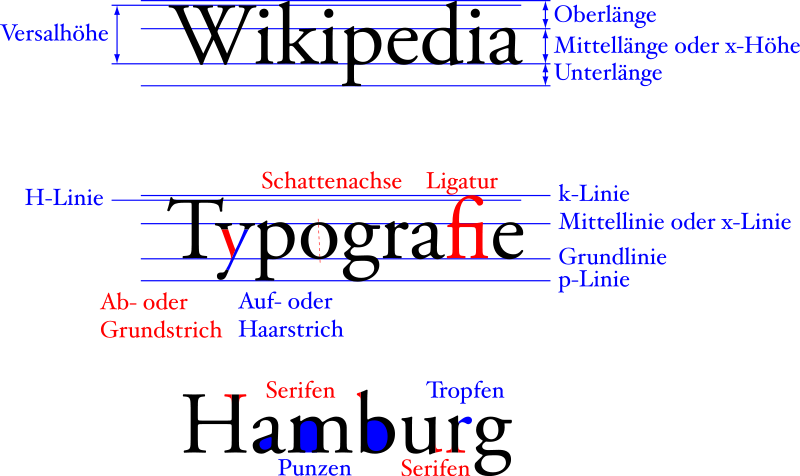
\includegraphics[height=130pt]{typografie.png}
\textit{(Bild: Brian Ammon, CC-BY)}
\end{center}
\begin{enumerate}
\item Höhe wird in Punkt angegeben. Ein Punkt ist meist 1/72 Zoll (TeX, DTP / Postscript), 1 Pica sind 12 Punkte.
\item Schrifstärke (manger, normal, fett), Schriftbreite (schmal, normal, breit), Schriftlage (normal, kursiv)
\item Vektorschriften: Definition durch Vektoren, Rasterschriften: Definition durch Pixelgrafik für je ein Zeichen
\item Serifen: Helfen bei Lesbarkeit, sollte nur bei Fließtext benutzt werden.
\item Kerning: Anpassung von Zeichenabständen bei parallelen Diagonalen ("BRAVO": Zusammenrücken von A und V), Definition pro Buchstabenpaar. Kann doof sein bei geringen Abständen. 
\end{enumerate}
\subsection{Absätze}
Absatzformat gibt Abstände und Einrückungen an. Möglich sind z. B. Blocksatz (Automatische Anpassung des Wortabstandes, sodass stets ganze Zeile gefüllt wird), Flattersatz / Mittelachsensatz (optimale Wortabstände). Seitenlayout: Kopf, Rumpf, Fuß. 
\subsection{Formate}
Eigenschaften: Editierbar? WYSISWG? Lesbar? Medien einbindbar? Funktionsumfang? Programmierbar?
\begin{itemize}
\item \textbf{Plain}
\item \textbf{Rich Text} (Microsoft), eigene Definition für Medien, nicht programmierbar, alt, WYSIWYG, MS Word, \LaTeX, PostScript, PDF, XHTML - \begin{lstlisting}
{\rtf Hallo \par {\i Dies} war kursiv.
\par Noch ne Zeile.}\end{lstlisting}
\item \LaTeX (Frei), voll programmierbar, kein WYSIWYG (wirft PDF o. ä. aus), Medien einbindbar, gute Formelsetzungsbibliotheken, vielseitig und toll, aber kompliziert
\item \textbf{PDF} (Adobe), baut auf Postscript auf, Layout-Treu, Rechtemanagment, Einbetten von Schriften problematisch, kaum editierbar, wird aus anderen Formatne generiert
\item \textbf{HTML}: Trennung von Struktur und Style mit CSS, Scripting (Document Object Model: Abbildung des XML-Baums auf JavaScript), programmierbar, kein WYSIWYG, Plugins
\end{itemize}
\section{Internetz}
\begin{itemize}
\item \textbf{HTTP}: Protokoll zwischen Web-Server und Web-Client (Browser)
\item \textbf{URI}: Bezeichnung und Adressierung beliebiger Daten im Netz (z. B. http://www.wh2.tu-dresden.de)
\item \textbf{Hypertext}: "Nicht-lineares" Textmedium, verbindet Inhalte durch Hyperlinks (URI, entfernte URIs wie "http://google.de", "ftp://..." oder lokale URIs wie "mailto:", die an andere Programme auf dem Rechner gehen)
\item \textbf{Mark-Up-Sprachen}: Beschreibung von Text durch Text, bspw. HTML mit öffnenden Tags und schließenden Tags und Inhalt dazwischen
\end{itemize}
\subsection{HTML}
\begin{lstlisting}
<html><head><title>Hallo Welt</title>
</head><body><h1>Grosse Ueberschrift
</h1><a href="uri">Link</a></body></html>
\end{lstlisting}
\begin{itemize}
\item Attribute bspw. href mit Ziel-URI, align mit Ausrichtung o. ä.
\item \lstinline|<a>|-Elemente sind Anker, verlinkt wird per \lstinline|"#ziel"| und gesetzt per name-Attribut
\item Bilder mit
\lstinline|<img src="uri" alt="beschreibung"|
\lstinline|width="300" height="300">|
\item Listen mit ul (unordered list) und ol (ordered list)-Elementen, Einträge mit li (list item)-Elementen
\item Tabellen mit table, tr für Zeilen und td für Spalten.
\begin{lstlisting}
<table><tr><th>1</th><th>2</th></tr>
<td>A</td><td>b</td></tr></table>
\end{lstlisting}
\item div für allgemeine Blöcke
\end{itemize}
\subsection{Barrierefreiheit}
Barrieren für Behinderte auf Webseiten (Sehbehinderte, Farbenblinde, Gehörbehinderte, Motorisch behińderte, geistig behinderte)
\subsection{CSS}
Strikte Trennung zwischen Präsentation und Design, definierte Formate für XHTML-Tags. Text-Formatierung, Positionierung von Elementen, Rahmen und Leerräume, Hintergrund, Formatierung von Tabellen, CSS einbinden mit \lstinline|<style type="text/css"></style>| für direktes Reinschreiben von CSS, CSS-Datei im Head des HTML-Dokuments verlinken mittels \lstinline|<link rel="stylesheet"| \lstinline|type="text/css" href="datei.css">|. HTML-Elemente koennen auch mit style-Attribut und CSS-Angaben gestyled werden.\\
CSS besteht aus Selektoren für Elemente (mittels ID oder Klasse) und Style-Attributen. Bspw.: \lstinline|#foo { color: red; }| setzt die Schriftfarbe im Element mit der ID foo auf rot. Mögliche Styleattribute sind z. B. "font-family" (Arial, sans-serif), "font-weight" (bold).\\
\subsection{Positionierung}
Mit CSS werden Elemente nach dem Boxmodel layoutet, d. h. jedes Element bildet eine Box. CSS-Attribute für jedes Element sind z. B. "margin" (Außenrand um die Box des Elements, z. B. "5px"), "padding" (Innenabstand um den Boxrand), "border-width" (Randbreite), "border-color" (Randfarbe).
\subsection{Navigationstechniken}
Websiten sollten sets einwandfrei navigierbar sein (vor / zurück, Nutzer muss sich zurechtfinden können). Bspw. durch Setzen von Navigationsleisten, Suchmaschinen etc.
\subsection{Karten in HTML}
Map-Element definiert Karte. Bsp.:
\begin{lstlisting}
<map name="schland">
<area shape="rect" cords="11,10,59,29"
href="uri" alt="Hier"></map>
<img src="map.png" usemap="#schland">
\end{lstlisting}
Beispielsweise rect mit coords="x1,y1,x2,y2" mit 1=Obere Linke Ecke,2=Untere rechte Ecke oder "circle" mit "x,y,r" oder "poly" "x1,y1,x2,y2..."
\section{Dynamisches Web}
Dynamik z. B. durch auf dem Web-Server dynamisch generierte Inhalte durch PHP, ASP.net o. ä. Im Browser wird JavaScript benutzt.
\subsection{JavaScript}
\begin{enumerate}
\item \textbf{Objekt}: Ein JavaScript-Objekt besteht aus Schlüsseln, denen Werte zugeordnet werden (bspw. das document-Objekt hat den Schlüssel bgcolor mit dem Wert white).
\item \textbf{Funktionen / Methoden / Aktionen}: Wie Funktionen in C, könnnen auch Variablen zugeordnet werden
\item \textbf{Ereignisse}: Das Ereignis "onmouseover" eines HTML-Elements kann durch JavaScript auf eine Funktion gesetzt werden.
\item \textbf{Variablen}: Können Zahlen, Strings, Booleans, Objekte, Funktionen sein. Bsp. zur Dekleration: \lstinline|var month = "Januar";|
\item Ausdrücke ordnen einer Variable einen Wert zu (Beispiel s. o.)
\item Operatoren verändern Variablen (siehe C, bspw. "+", "==")
\end{enumerate}
\rule{0.3\linewidth}{0.25pt}
\scriptsize

Gebaut mit \LaTeX

\end{multicols}
\end{document}